\chapter{Σχεδίαση και αρχιτεκτονική λογισμικού}
\label{ch:architecture}
Στην ενότητα αυτή θα περιγραφούν τα βασικά συστατικά του συστήματος
 καθώς και οι σχέσεις που τα συνδέουν μεταξύ τους.
\section{Πακέτα συστήματος}
\label{sec:packages}
\begin{figure}[H]
    \centering
    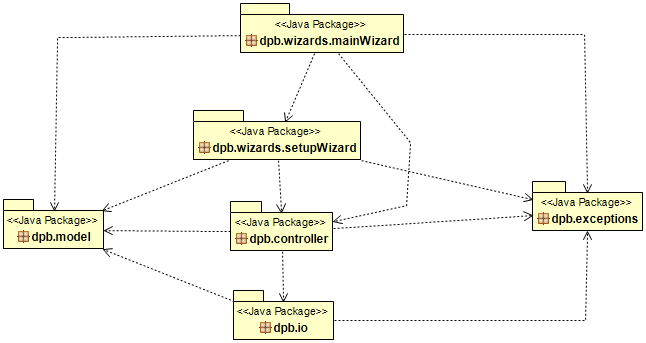
\includegraphics[width=1.0\textwidth]{Figures/packages.png}
    \label{fig:packageUML}
    \caption{Διάγραμμα UML Πακέτων συστήματος}
\end{figure}
Το λογισμικό αποτελείται από τα παρακάτω πακέτα,
\begin{itemize}
    \item dpb.wizards.mainWizard, σε αυτό το πακέτο, περιέχονται οι κλάσεις που αφορούν το γραφικό περιβάλλον του εργαλείου,
     πιο συγκεκριμένα, οι κλάσεις αυτού του πακέτου έχουν να κάνουν με την επιλογή του μοτίβου και την διαχείριση των κλάσεων και διεπαφών του 
     επιλεγμένου μοτίβου
    \item dpb.wizards.setupWizards, σε αυτό το πακέτο, υπάρχουν οι κλάσεις που έχουν σχέση με την γραφική διεπαφή και την τροποποίηση των κλάσεων και διεπαφών, 
    όπως και των μεθόδων και πεδίων
    \item dpb.controller, αποτελεί το πακέτο μέσω του οποίου η γραφική διεπαφή επικοινωνεί με το back-end. Χρησιμοποιεί τις λειτουργίες που παρέχει το back-end, 
    ώστε να  μετασχηματίζει τα ακατέργαστα δεδομένα των μοτίβων που παίρνει από το υποσύστημα io σε αντικείμενα κλάσεων που παρέχει το πακέτο model
    \item dpb.io, αποτελεί το κομμάτι του συστήματος το οποίο χαρακτηρίζεται ως back-end
     και είναι υπεύθυνο για το διάβασμα του αρχείου xml στο οποίο περιγράφονται τα μοτίβα. Παρέχει λειτουργίες για την εισαγωγή των μοτίβων στο σύστημα
    \item dpb.model, Το πακέτο αυτό, περιέχει τις κλάσεις οι οποίες αναπαριστούν τα αντικείμενα του πεδίου του προβλήματος
    \item dpb.exceptions, Τέλος, στο πακέτο αυτό υπάρχουν κάποιες κλάσεις οι οποίες αναπαριστούν εξαιρέσεις 
    οι οποίες είναι κάποια γεγονότα που συμβαίνουν κατά την εκτέλεση του εργαλείου και διακόπτουν την κανονική ροή του προγράμματος.
\end{itemize}
\newpage
\section{Κλάσεις συστήματος}
\label{sec:classes}
\subsection{Ανάλυση κλάσεων}
\label{subsec:classAnalysis}
Παρακάτω, θα αναλύσουμε κάποιες βασικές κλάσεις του συστήματος,
\begin{itemize}
    \item PatternClass, η κλάση αυτή ανήκει στο πακέτο model και μοντελοποιεί μία κλάση του μοτίβου
    \item PatternInterface, η κλάση αυτή ανήκει στο πακέτο model και μοντελοποιεί μία διεπαφή του μοτίβου
    \item Method, η κλάση αυτή ανήκει στο πακέτο model και μοντελοποιεί μία μέθοδο που ανήκει σε κλάση ή διεπαφή του μοτίβου
    \item Field, η κλάση αυτή ανήκει στο πακέτο model και μοντελοποιεί ένα πεδίο που ανήκει σε κλάση του μοτίβου
    \item FileParser, είναι η βασική κλάση του υποσυστήματος io, είναι υπεύθυνη για το διάβασμα του αρχείου όπου περιγράφονται
    τα μοτίβα και η βασική της δουλειά είναι να διαβάζει το αρχείο xml. Υποστηρίζει λειτουργίες όπως η ανάκτηση 
    των κατηγοριών και των μοτίβων κάθε κατηγορίας, η ανάκτηση των κλάσεων και διεπαφών ενός μοτίβου, 
    η ανάκτηση των annotations κάθε στοιχείου για κάποιο μοτίβο, όπως και οι ιδιότητες ενός μοτίβου 
    οι οποίες είναι εάν επιτρέπεται η εισαγωγή νέας κλάσης, τέλος υποστηρίζει την ανάκτηση μεθόδων και πεδίων.
    \item PatternManager, Μέσω της κλάσης αυτής παρέχεται η δυνατότητα στην γραφική διεπαφή του συστήματος 
    να αντλεί οτιδήποτε χρειάζεται από το υποσύστημα io
    \item PatternGenerator, Περιλαμβάνει την λειτουργία δημιουργίας των πηγαίων αρχείων στο πακέτο του έργου που έχει επιλέξει 
    ο προγραμματιστής ή στο προεπιλεγμένο πακέτο, εάν δεν έχει επιλέξει κάποιο πακέτο, τα οποία περιέχουν 
    τις κλάσεις του μοτίβου με τις μεθόδους και τα πεδία, όπως τα παραμετροποίησε ο προγραμματιστής, καθώς και τις διεπαφές. 
    Επίσης προσθέτει στο classpath του έργου του προγραμματιστή το πακέτο που περιέχει τα annotations 
    ώστε να είναι διαθέσιμα στον προγραμματιστή.
     
\end{itemize}
\subsection{Διάγραμμα κλάσεων}
\begin{figure}[H]
    \centering
    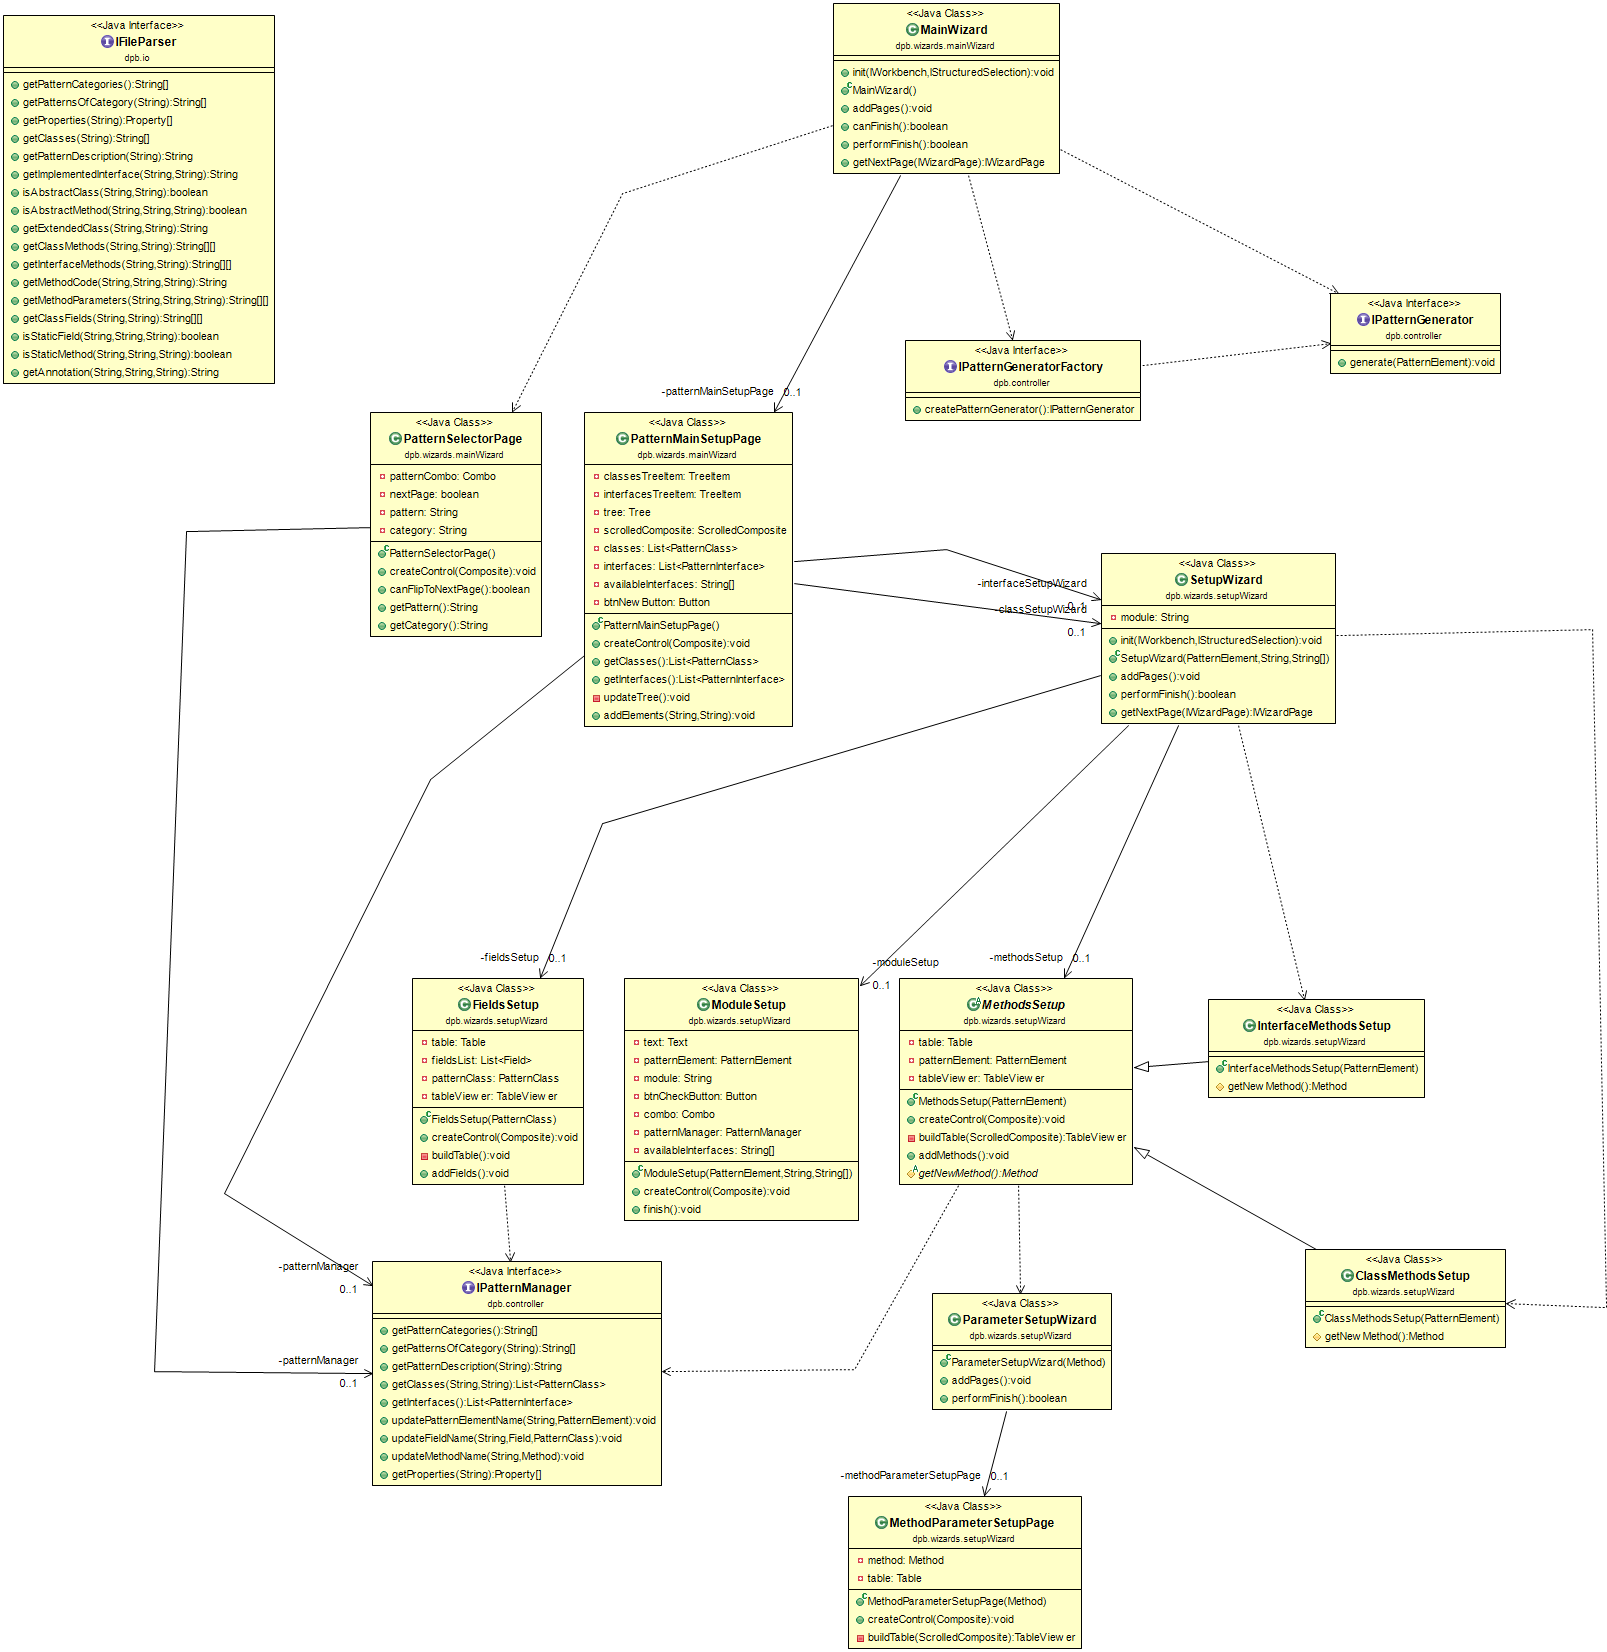
\includegraphics[width=0.9\textwidth]{Figures/system.png}
    \label{fig:systemUML}
    \caption{Διάγραμμα UML βασικών κλάσεων \& διεπαφών συστήματος}
\end{figure}
\begin{figure}[H]
    \centering
    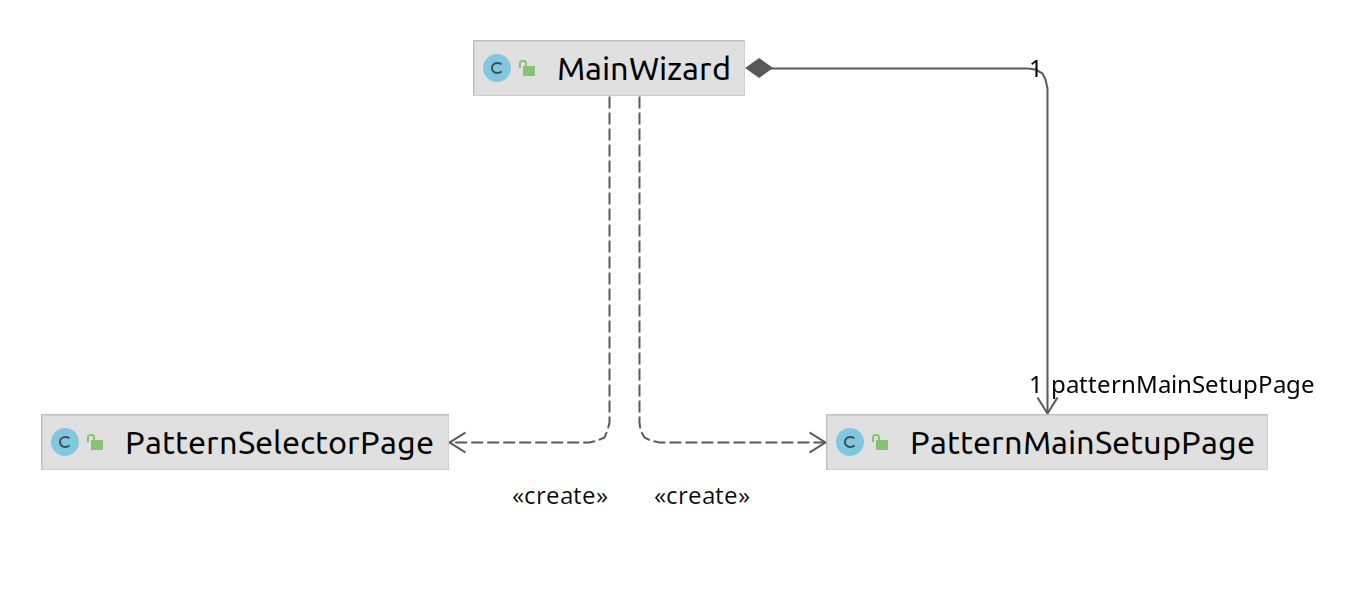
\includegraphics[width=0.7\textwidth]{Figures/mainWizard.png}
    \label{fig:mainWizardUML}
    \caption{Διάγραμμα UML Πακέτου mainWizard}
\end{figure}
\begin{figure}[H]
    \centering
    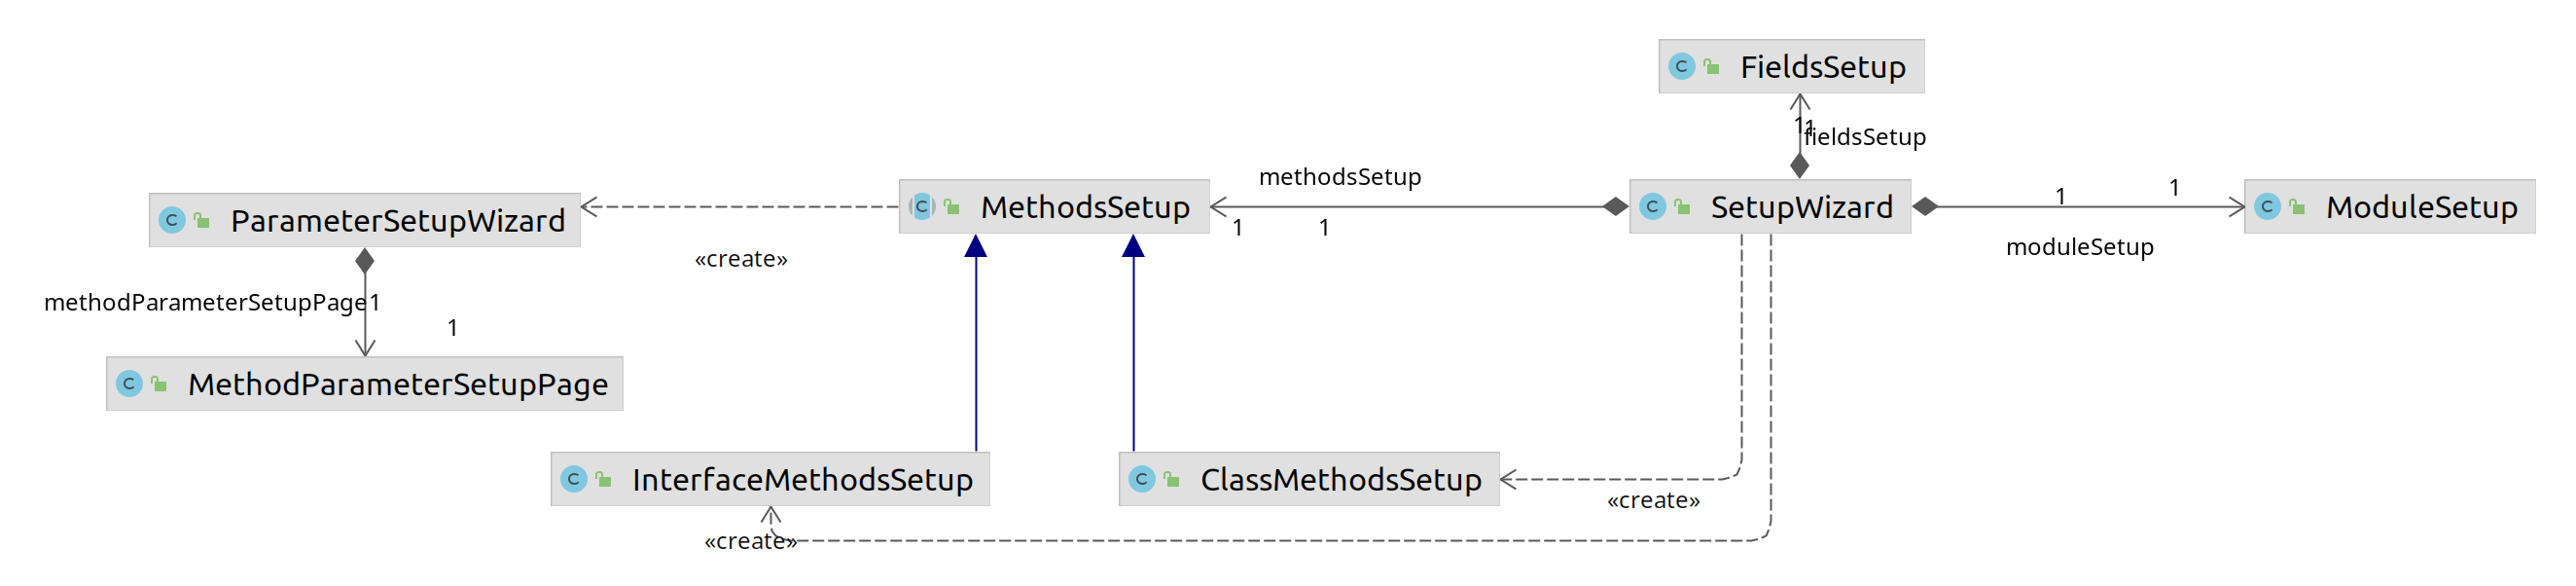
\includegraphics[width=0.9\textwidth]{Figures/setupWizard.png}
    \label{fig:setupWizardUML}
    \caption{Διάγραμμα UML Πακέτου setupWizards}
\end{figure}
\newpage
\begin{figure}[H]
    \centering
    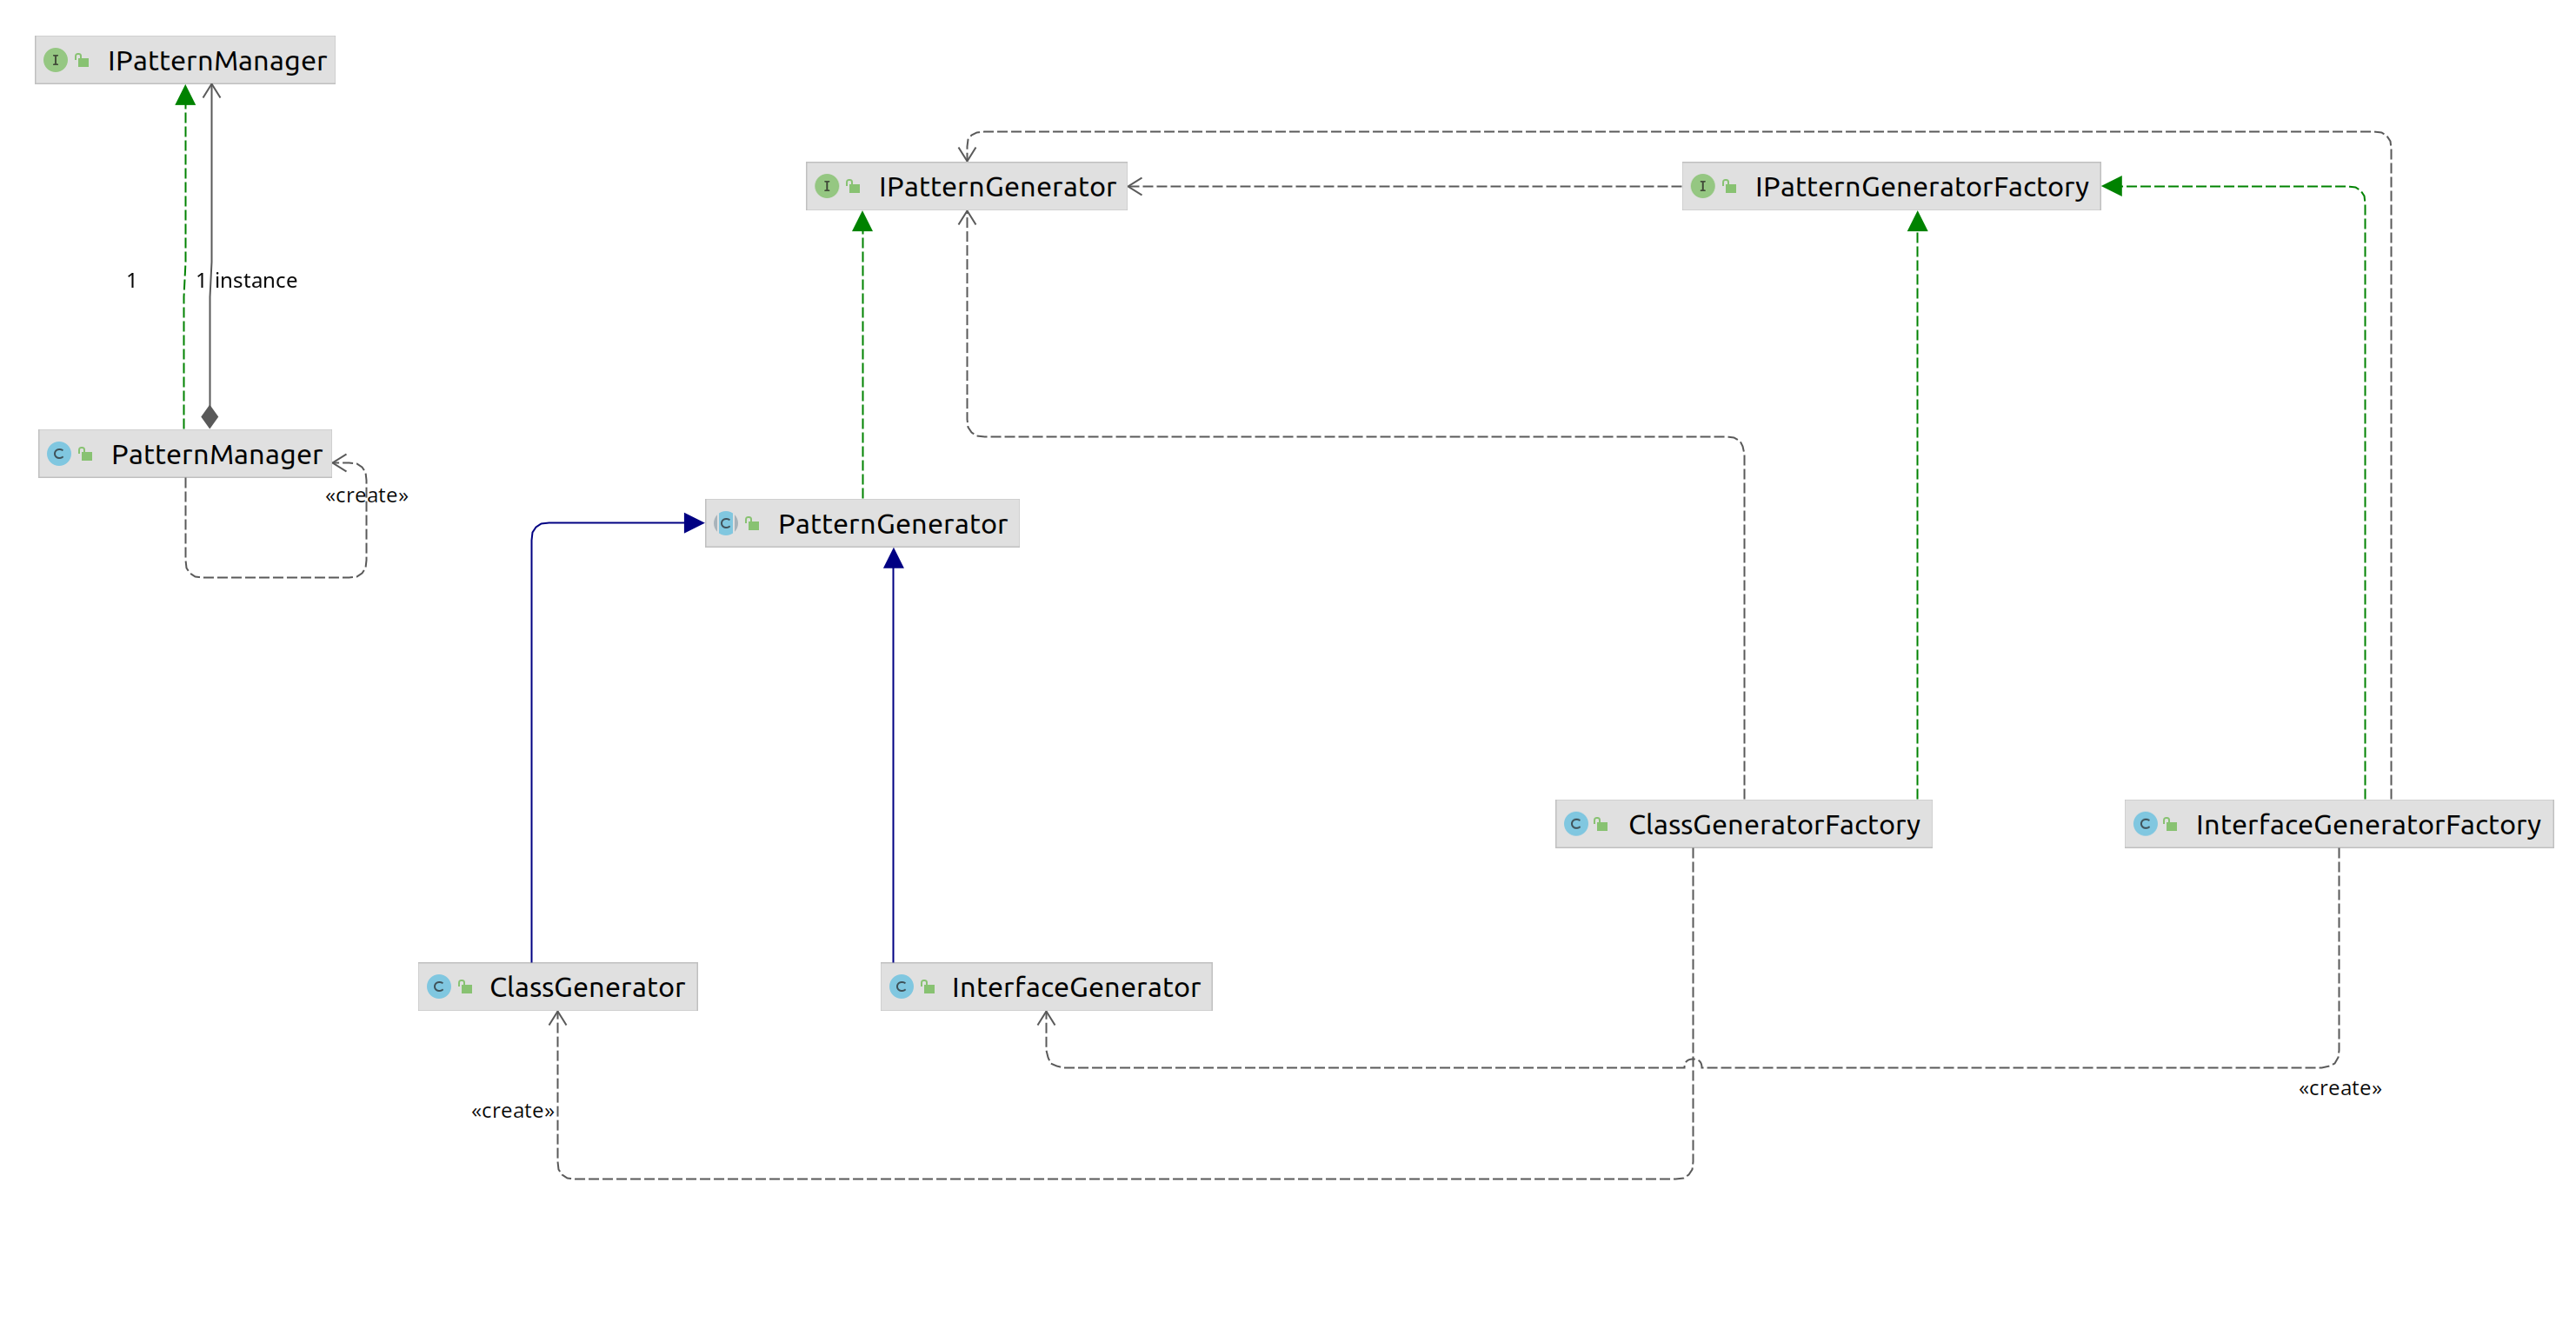
\includegraphics[width=1.0\textwidth]{Figures/controller.png}
    \label{fig:controllerUML}
    \caption{Διάγραμμα UML Πακέτου controller}
\end{figure}
\begin{figure}[H]
    \centering
    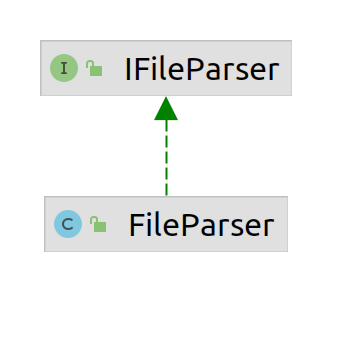
\includegraphics[width=0.4\textwidth]{Figures/io.png}
    \label{fig:ioUML}
    \caption{Διάγραμμα UML Πακέτου io}
\end{figure}
\begin{figure}[H]
    \centering
    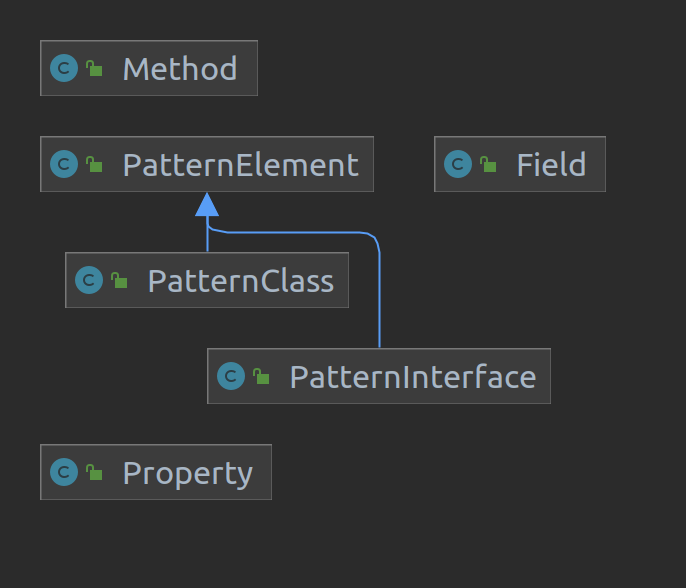
\includegraphics[width=1.0\textwidth]{Figures/model.png}
    \label{fig:modelUML}
    \caption{Διάγραμμα UML Πακέτου model}
\end{figure}
\label{subsec:ClassUML}
\section{Κάρτες αρμοδιοτήτων και συνεργασιών κλάσεων}
\label{sec:crc}
\begin{table}[H]
    \centering
    \begin{tabular}{|p{5cm}|p{5cm}|}
        \hline
        \multicolumn{2}{|l|}{Όνομα κλάσης: PatternClass} \\
        \hline
        \textbf{Αρμοδιότητες} & \textbf{Συνεργασίες} \\
        \hline
        \begin{itemize}
            \item Αυτή η κλάση είναι υπεύθυνη για την μοντελοποίηση μίας κλάσης ενός μοτίβου.
        \end{itemize} &   
        \begin{itemize}
            \item Method
            \item Field
        \end{itemize} \\
        \hline
    \end{tabular}
    \label{tab:PatternClassCRC}
    \caption{PatternClass κάρτα αρμοδιοτήτων}
\end{table}
\begin{table}[H]
    \centering
    \begin{tabular}{|p{5cm}|p{5cm}|}
        \hline
        \multicolumn{2}{|l|}{Όνομα κλάσης: PatternInterface} \\
        \hline
        \textbf{Αρμοδιότητες} & \textbf{Συνεργασίες} \\
        \hline
        \begin{itemize}
            \item Αυτή η κλάση είναι υπεύθυνη για την μοντελοποίηση μίας διεπαφής ενός μοτίβου.
        \end{itemize} &   
        \begin{itemize}
            \item Method
        \end{itemize} \\
        \hline
    \end{tabular}
    \label{tab:PatternInterfaceCRC}
    \caption{PatternInterface κάρτα αρμοδιοτήτων}
\end{table}
\begin{table}[H]
    \centering
    \begin{tabular}{|p{5cm}|p{5cm}|}
        \hline
        \multicolumn{2}{|l|}{Όνομα κλάσης: Method} \\
        \hline
        \textbf{Αρμοδιότητες} & \textbf{Συνεργασίες} \\
        \hline
        \begin{itemize}
            \item Η κλάση αυτή διατηρεί τα χαρακτηριστικά μίας μεθόδου που ανήκει σε κάποια κλάση ή διεπαφή.
        \end{itemize} &    
        % \begin{itemize}
        %     \item hi
        % \end{itemize} 
        \\
        \hline
    \end{tabular}
    \label{tab:MethodCRC}
    \caption{Method κάρτα αρμοδιοτήτων}
\end{table}
\begin{table}[H]
    \centering
    \begin{tabular}{|p{5cm}|p{5cm}|}
        \hline
        \multicolumn{2}{|l|}{Όνομα κλάσης: Field} \\
        \hline
        \textbf{Αρμοδιότητες} & \textbf{Συνεργασίες} \\
        \hline
        \begin{itemize}
            \item Η κλάση αυτή διατηρεί τα χαρακτηριστικά ενός πεδίου που ανήκει σε κάποια κλάση.
        \end{itemize} &   
        % \begin{itemize}
        %     \item hi
        % \end{itemize} 
        \\
        \hline
    \end{tabular}
    \label{tab:FieldCRC}
    \caption{Field κάρτα αρμοδιοτήτων}
\end{table}
\begin{table}[H]
    \centering
    \begin{tabular}{|p{10cm}|p{5cm}|}
        \hline
        \multicolumn{2}{|l|}{Όνομα κλάσης: FileParser} \\
        \hline
        \textbf{Αρμοδιότητες} & \textbf{Συνεργασίες} \\
        \hline
        \begin{itemize}
            \item Η κλάση αυτή είναι υπεύθυνη για την άντληση των κατηγοριών που ορίζουν οι GoF \cite{GoF}.
            \item Η κλάση αυτή αρμόδια για την άντληση των μοτίβων κάποιας κατηγορίας.
            \item Η κλάση αυτή είναι αρμόδια για την άντληση των κλάσεων ενός μοτίβου, όπως και την ορατότητα της κλάσης.
            \item Η κλάση αυτή είναι αρμόδια για την άντληση των διεπαφών ενός μοτίβου όπως και την ορατότητα της διεπαφής.
            \item Η κλάση αυτή είναι αρμόδια για την άντληση των μεθόδων κάποιας κλάσης, καθώς τους διάφορους τροποποιητές που μπορεί 
            να έχει μία μέθοδος, όπως και τον επιστρεφόμενο τύπο της μεθόδου και τέλος τον κώδικα της μεθόδου.
            \item Η κλάση αυτή είναι αρμόδια για την άντληση των πεδίων κάποιας κλάσης ενός μοτίβου.
            \item Η κλάση αυτή είναι αρμόδια για την άντληση των μεθόδων κάποιας διεπαφής μαζί με τους 
            τροποποιητές της μεθόδου και τον επιστρεφόμενο τύπο της.
            \item Η κλάση αυτή είναι αρμόδια για την άντληση των annotations ενός στοιχείου του μοτίβου.
        \end{itemize} &   
        % \begin{itemize}
        %     \item 
        % \end{itemize}
         \\
        \hline
    \end{tabular}
    \label{tab:fileParserCRC}
    \caption{FileParser κάρτα αρμοδιοτήτων}
\end{table}
\begin{table}[H]
    \centering
    \begin{tabular}{|p{10cm}|p{5cm}|}
        \hline
        \multicolumn{2}{|l|}{Όνομα κλάσης: PatternManager} \\
        \hline
        \textbf{Αρμοδιότητες} & \textbf{Συνεργασίες} \\
        \hline
        \begin{itemize}
            \item Η κλάση αυτή είναι αρμόδια για την διάθεση των κατηγοριών των μοτίβων στην γραφική διεπαφή.
            \item Η κλάση αυτή είναι αρμόδια για την διάθεση των μοτίβων κάποιας κατηγορίας στην γραφική διεπαφή.
            \item Η κλάση αυτή είναι αρμόδια για την δημιουργία αντικειμένων τύπου PatternClass και την διαθέση τους στο front-end τμήμα του 
            εργαλείου, ώστε να μπορεί να διαχειριστεί ο χρήστης τις διάφορες κλάσεις ενός μοτίβου.
            \item Η κλάση αυτή είναι αρμόδια για την δημιουργία αντικειμένων τύπου PatternInterface και την διαθέση τους στο front-end τμήμα του 
            εργαλείου, ώστε να μπορεί να διαχειριστεί ο χρήστης τις διάφορες διεπαφές ενός μοτίβου.
            \item Η κλάση αυτή είναι αρμόδια για την ενημέρωση του ονόματος μίας κλάσης.
            \item Η κλάση αυτή είναι αρμόδια για την ενημέρωση του ονόματος μίας διεπαφής.
            \item Η κλάση αυτή είναι αρμόδια για την ενημέρωση του ονόματος μίας μεθόδου.
            \item Η κλάση αυτή είναι αρμόδια για την ενημέρωση του ονόματος ενός πεδίου.
        \end{itemize} &   
        \begin{itemize}
            \item FileParser
            \item PatternClass
            \item PatternInterface
            \item Method
            \item Field
            \item Property
        \end{itemize} \\
        \hline
    \end{tabular}
    \label{tab:PatternManagerCRC}
    \caption{PatternManager κάρτα αρμοδιοτήτων}
\end{table}
\begin{table}[H]
    \centering
    \begin{tabular}{|p{5cm}|p{5cm}|}
        \hline
        \multicolumn{2}{|l|}{Όνομα κλάσης: ClassGenerator} \\
        \hline
        \textbf{Αρμοδιότητες} & \textbf{Συνεργασίες} \\
        \hline
        \begin{itemize}
            \item Η κλάση αυτή είναι αρμόδια για την προσθήκη των annotations στο classpath του έργου που έχει επιλέξει ο προγραμματιστής.
            \item Η κλάση αυτή είναι αρμόδια για την παραγωγή των πηγαίων αρχείων java μίας κλάσης.
        \end{itemize} &   
        \begin{itemize}
            \item PatternManager
            \item PatternClass
            \item PatternInterface
            \item Method
            \item Field
            \item Property
        \end{itemize} \\
        \hline
    \end{tabular}
    \label{tab:ClassGeneratorCRC}
    \caption{ClassGenerator κάρτα αρμοδιοτήτων}
\end{table}
\begin{table}[H]
    \centering
    \begin{tabular}{|p{5cm}|p{5cm}|}
        \hline
        \multicolumn{2}{|l|}{Όνομα κλάσης: InterfaceGenerator} \\
        \hline
        \textbf{Αρμοδιότητες} & \textbf{Συνεργασίες} \\
        \hline
        \begin{itemize}
            \item Η κλάση αυτή είναι αρμόδια για την προσθήκη των annotations στο classpath του έργου που έχει επιλέξει ο προγραμματιστής.
            \item Η κλάση αυτή είναι αρμόδια για την παραγωγή των πηγαίων αρχείων java μίας διεπαφής.
        \end{itemize} &   
        \begin{itemize}
            \item PatternManager
            \item PatternClass
            \item PatternInterface
            \item Method
            \item Field
            \item Property
        \end{itemize} \\
        \hline
    \end{tabular}
    \label{tab:InterfaceGeneratorCRC}
    \caption{InterfaceGenerator κάρτα αρμοδιοτήτων}
\end{table}